\documentclass[12pt,a4paper]{article}
\usepackage{amsmath,amssymb,makecell,fancyhdr,enumerate,arcs,physics,tasks,mathrsfs,graphics}
\usepackage{tikz,tikz-3dplot,tkz-euclide,tkz-tab,tabvar,pgfplots,esvect}
\usepackage[top=1.5cm, bottom=1.5cm, left=2cm, right=1.5cm]{geometry}
\usepackage[hidelinks,unicode]{hyperref}
\usepackage[utf8]{vietnam}
\usepackage{polyglossia}
\usepackage[loigiai]{ex_test}
\usepackage{lastpage}
\usepackage{diagbox}
\usepackage{fontawesome5}
\usetikzlibrary{shapes.geometric,shadings,calc,snakes,patterns,arrows,intersections,angles,backgrounds,quotes}
\usepgfplotslibrary{fillbetween}
\pgfplotsset{compat=newest}
\tikzset{point style/.append style={color=white}}
\def\vec{\overrightarrow}
\newcommand{\hoac}[1]{\left[\begin{aligned}#1\end{aligned}\right.}
\newcommand{\heva}[1]{\left\{\begin{aligned}#1\end{aligned}\right.}
\newcommand{\hetde}{\centerline{\rule[0.5ex]{2cm}{1pt} HẾT \rule[0.5ex]{2cm}{1pt}}}
\newcommand{\tentruong}{TRƯỜNG THPT NGUYỄN HỮU CẢNH}
\newcommand{\tengv}{GV Nguyễn Văn Sang}
\newcommand{\tenkythi}{KIỂM TRA HKI NĂM HỌC 2025-2026}
\newcommand{\tenmonthi}{MÔN TOÁN - LỚP 12}
\newcommand{\thoigian}{90}
\newcommand{\tieude}[3]{
    \noindent
    \begin{minipage}[b]{7cm}
        \centerline{\textbf{\fontsize{13}{0}\selectfont \tentruong}}
        \centerline{\textbf{\fontsize{13}{0}\selectfont \tengv}}
        \centerline{(\textit{Đề thi có #1 trang})}
        \centerline{\textit{ }}
    \end{minipage}\hspace{1.5cm}
    \begin{minipage}[b]{9cm}
        \centerline{\textbf{\fontsize{13}{0}\selectfont \tenkythi}}
        \centerline{\textbf{\fontsize{13}{0}\selectfont \tenmonthi}}
        \centerline{\textit{\fontsize{12}{0}\selectfont Thời gian làm bài \thoigian \ phút}}
        \centerline{\textit{\fontsize{12}{0}\selectfont (Đề có 12 câu trắc nghiệm, 4 đúng sai, 6 điền đáp án)}}
    \end{minipage}
    \begin{minipage}[b]{13cm}
        \vspace*{.75cm}
        \textbf{Họ và tên thí sinh: }{\tiny\dotfill}\\
        \textbf{Số Báo Danh: }{\tiny\dotfill}
    \end{minipage}
    \begin{minipage}[b]{8cm}
        \hspace*{1cm}\fbox{\bf Mã đề thi #3}
    \end{minipage}
}
\newcommand{\chantrang}[2]{\rfoot{Trang \thepage/\pageref{LastPage} $-$ Mã đề #2}}
\pagestyle{fancy}
\fancyhf{}
\renewcommand{\headrulewidth}{0pt}
\def\colorEX{}
\renewtheorem{ex}{\color{blue!80!black}\textbf{Câu}}

\newcommand{\made}{222}
\usepackage{polyglossia}
\begin{document}
\tieude{\pageref{LastPage}}{0}{\made}
\chantrang{\pageref{LastPage}}{\made}
%\begin{center}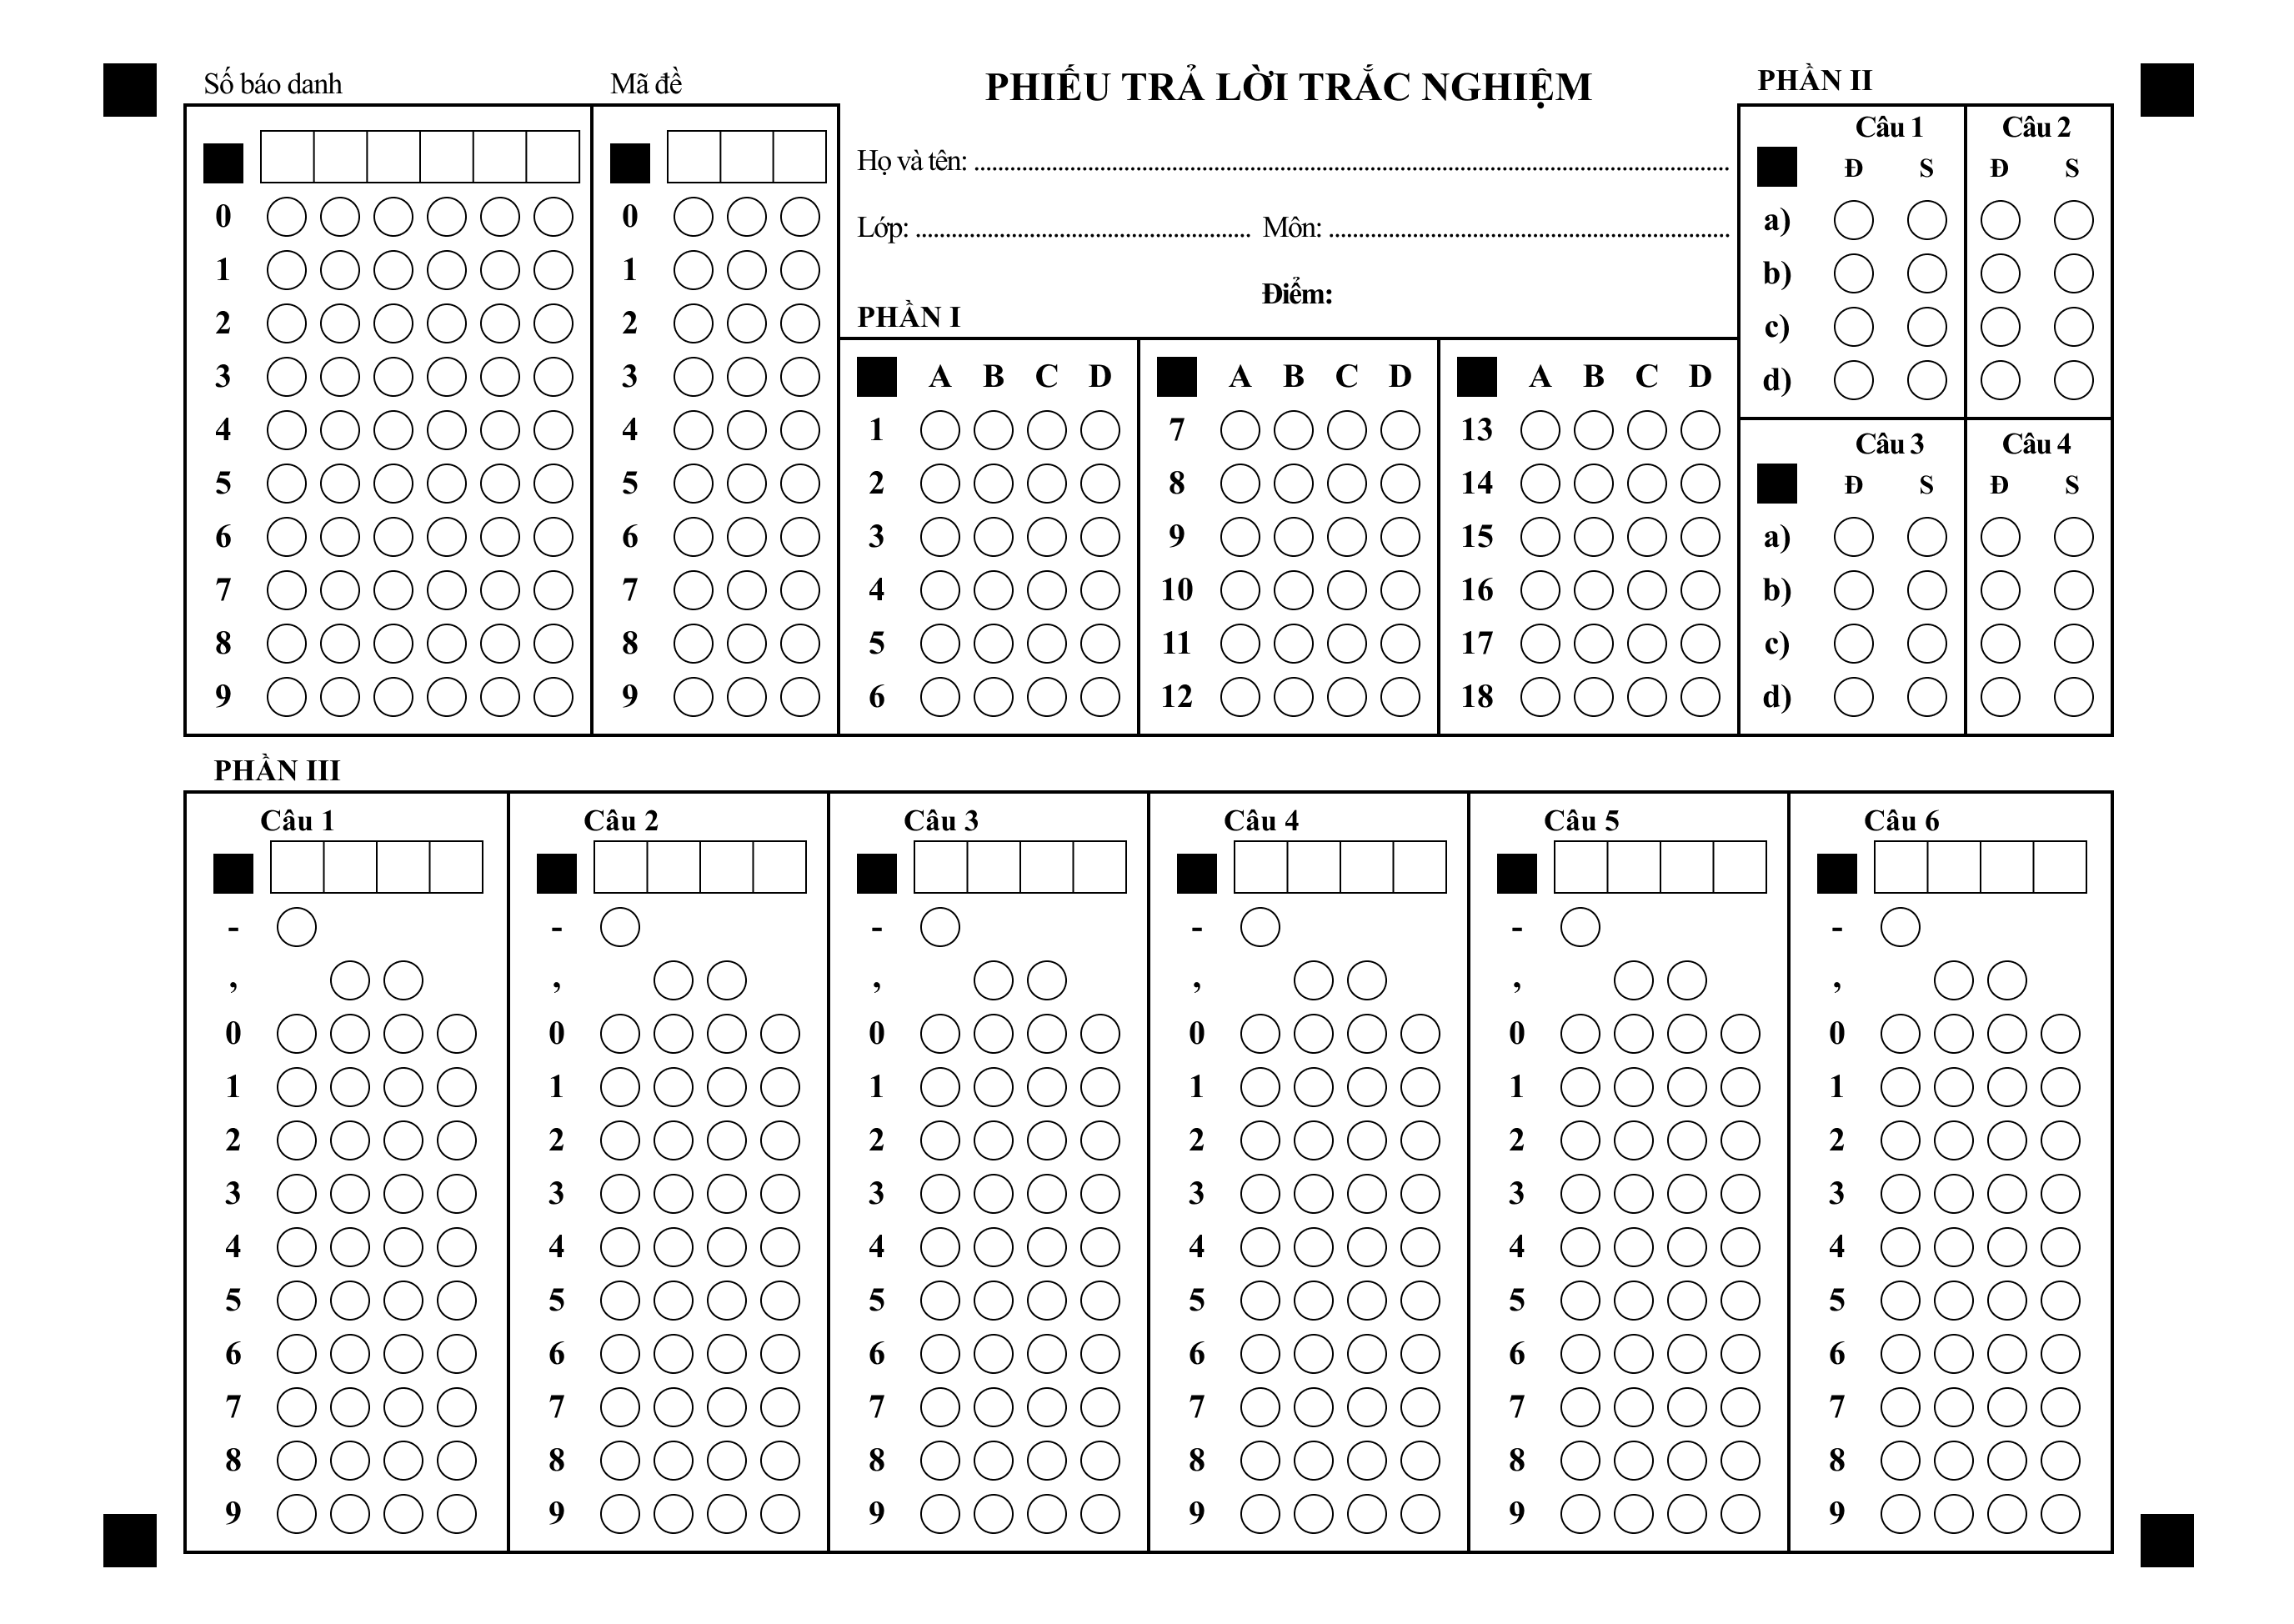
\includegraphics[width=1\textwidth]{UnT18.4.6.png}\end{center}
\subsection*{PHẦN I. Trắc nghiệm nhiều lựa chọn. (12 câu)}
\setcounter{ex}{0}
\Opensolutionfile{ans}%%[ans-phanI]
\begin{ex}%[2D3H2-2]%[CTST - Lớp 12 - THPT Thiên Phước - Đồng Nai]%[Dương Công Tạo]
	Bảng sau thống kê số lượt khách mỗi ngày của một hãng taxi trong $30$ ngày
	\begin{center}
		\begin{tabular}{|l|c|c|c|c|c|}
		\hline
		Số lượt & {$[5; 8)$} & $(8;11)$ & $11; 14)$ & $14; 17)$ & $(17;20)$ \\
		\hline
		Số ngày & 4 & 9 & 9 & 5 & 3\\
		\hline
	\end{tabular}
	\end{center}
	Độ lệch chuẩn $S$ của mẫu số liệu trên thỏa
	\choice
{\True $3< S< 4$}
{$1< S< 2$}
{$2< S< 3$}
{$4< S< 5$}
	\loigiai{
		\begin{center}
			\begin{tabular}{|l|c|c|c|c|c|}
				\hline
				Số lượt & $[5; 8)$ & $(8;11)$ & $11; 14)$ & $14; 17)$ & $(17;20)$ \\
				\hline
				Giá trị đại diện & $6{,}5$ & $9{,}5$ & $12{,}5$ & $15{,}5$ & $18{,}5$ \\
				\hline
				Số ngày & 4 & 9 & 9 & 5 & 3\\
				\hline
			\end{tabular}
		\end{center}
		Số khách trung bình trong $30$ ngày 
		\begin{align*}
			\overline{x}=\dfrac{1}{30}\left(6{,}5\cdot 4+9{,}5\cdot 9+12{,}5\cdot 9+15{,}5\cdot5+18{,}5\cdot 3\right)=11{,}9\text{ (khách)}.
		\end{align*}
		Phương sai của mẫu số liệu trên là 
		\begin{align*}
			S^2=&\dfrac{1}{30}[(6{,}5-11{,}9)^2\cdot 4+(9{,}5-11{,}9)^2\cdot 9+(12{,}5-11{,}9)^2\cdot 9+\\&(15{,}5-11{,}9)^2\cdot5+(18{,}5-11{,}9)^2\cdot 3]=12{,}24.
		\end{align*}
	Vậy độ lệch chuẩn $S$ của mẫu số liệu trên là $S\approx3{,}5$.
	}
\end{ex}

\subsection*{PHẦN II. Trắc nghiệm đúng sai. (4 câu)}
\setcounter{ex}{0}
\Opensolutionfile{ans}%%[ans-phanII]
\begin{ex}%[2H2H2-4]%[2-TN-DS-TLN-THPT-ThienPhuoc-DongNai-HKI-NH24-25 - Phúc Chương]
	Trong không gian $Oxyz$, cho $\overrightarrow{a}=(-2;2;1)$, $\overrightarrow{b}=(-1;1;3)$.
	\choiceTF
{$2\overrightarrow{a}-\overrightarrow{b}$ có toạ độ $(-3;3;1)$}
{\True $\cos\left(\overrightarrow{a},\overrightarrow{b}\right)=\dfrac{7\sqrt{11}}{33}$}
{\True $\overrightarrow{u}=(5;-5;0)$ vuông góc với cả $2$ vectơ $\overrightarrow{a}$, $\overrightarrow{b}$}
{\True $\left|\overrightarrow{a}\right|=3$}
	\loigiai{
		\begin{itemchoice}
			\itemch \textbf{Đúng}.\\
			Ta có $\left|\vec{a}\right|=\sqrt{(-2)^2+2^2+1}=3$.
			\itemch \textbf{Sai}.\\
			Ta có $2\vec{a}-\vec{b}=\left(2a_1-b_1;2a_2-b_2;2a_3-b_3\right)=(-3;3;-1)$.
			\itemch \textbf{Đúng}.\\
			Ta có $\cos\left(\vec{a},\vec{b}\right)=\dfrac{\vec{a}\cdot\vec{b}}{\left|\vec{a}\right|\cdot\left|\vec{b}\right|}=\dfrac{7}{3\cdot\sqrt{11}}=\dfrac{3\sqrt{11}}{33}$.
			\itemch \textbf{Đúng}.\\
			Ta có $\vec{u}\cdot\vec{a}=0$ và $\vec{u}\cdot\vec{b}=0$, suy ra $\vec{u}\perp\vec{a}$ và $\vec{u}\perp\vec{b}$.
		\end{itemchoice}
	}
\end{ex}
\Closesolutionfile{ans}%%%
\end{document}
